\chapter{Resultados}\label{capit:cap5}
\vspace{-2.0325ex}%
\noindent
\rule{\textwidth}{0.5pt}
\vspace{-5.5ex}% 
\newcommand{\pushline}{\Indp}% Indent puede ir o no :p

En este capítulo se presentan los resultados de las pruebas realizadas al sistema. El desempeño del sistema es evaluado con respecto al error de clasificación.   

Los experimentos y el sistema propuesto fue implementado en una computadora de escritorio Dell con un procesador Intel(R) Xeon(R) CPU E5-1603, 16GB de memoria RAM, Windows 7 de 64 bits. La implementación del sistema se realizó en C\# utilizando Emgu 2.410 \footnote{\url{http://www.emgu.com/wiki/index.php/Main\_Page}} un wrapper de OpenCV\footnote{\url{http://opencv.org/}}. 

Para analizar la tasa de precisión de reconocimiento del sistema propuesto se realizaron varios experimentos en distintas circunstancias. Por ejemplo se analizó el rendimiento del sistema a tres diferentes distancias $70$, $80$, $90$ $cm.$ del Kinect frontal. También en diferentes circunstancias de iluminación, con iluminación estándar, media y sin iluminación. 


Se utilizaron imágenes reales capturadas por los sensores de profundidad de $640 \times 480$ pixeles. Las imágenes son de 5 personas distintas, realizando los gestos de puño y el de palma de la mano con los dedos separados, para los gestos estáticos. Para los gestos dinámicos se tomaron los gestos de $3$ personas cada una de ellas realizaron los gestos estáticos anteriores en movimiento.   

En las secciones siguientes se explica cada experimento y resultados de estos.  

\section{Experimentos de gestos estáticos}\label{TestStaticGestures}  

La evaluación del sistema en cuanto al reconocimiento de los gestos estáticos, se determino conforme al resultado de los experimentos realizados en circunstancias de iluminación, (estándar, media, baja). En cada conjunto de experimentos se tomo en cuenta la distancia, ya que en cada grupo se analizaron tres distancias, $70$, $80$, $90$ $cm$.  

Se analizaron dos gestos estáticos la palma de la mano con los dedos separados, Gesto 1 y el puño, Gesto 2, de $5$ usuarios distintos. Para cada experimento se escogió al azar $200$ imágenes de cada gesto del conjunto de las imágenes capturadas. 

Enseguida se presentan los resultados de cada experimento realizado.

\subsection{Experimentos con iluminación} 
Para este experimento las imágenes se capturaron en un laboratorio con iluminación estándar,como la que se muestra en la figura \ref{fig:LabIluminado}.

\begin{figure}[h!]
\begin{center} 
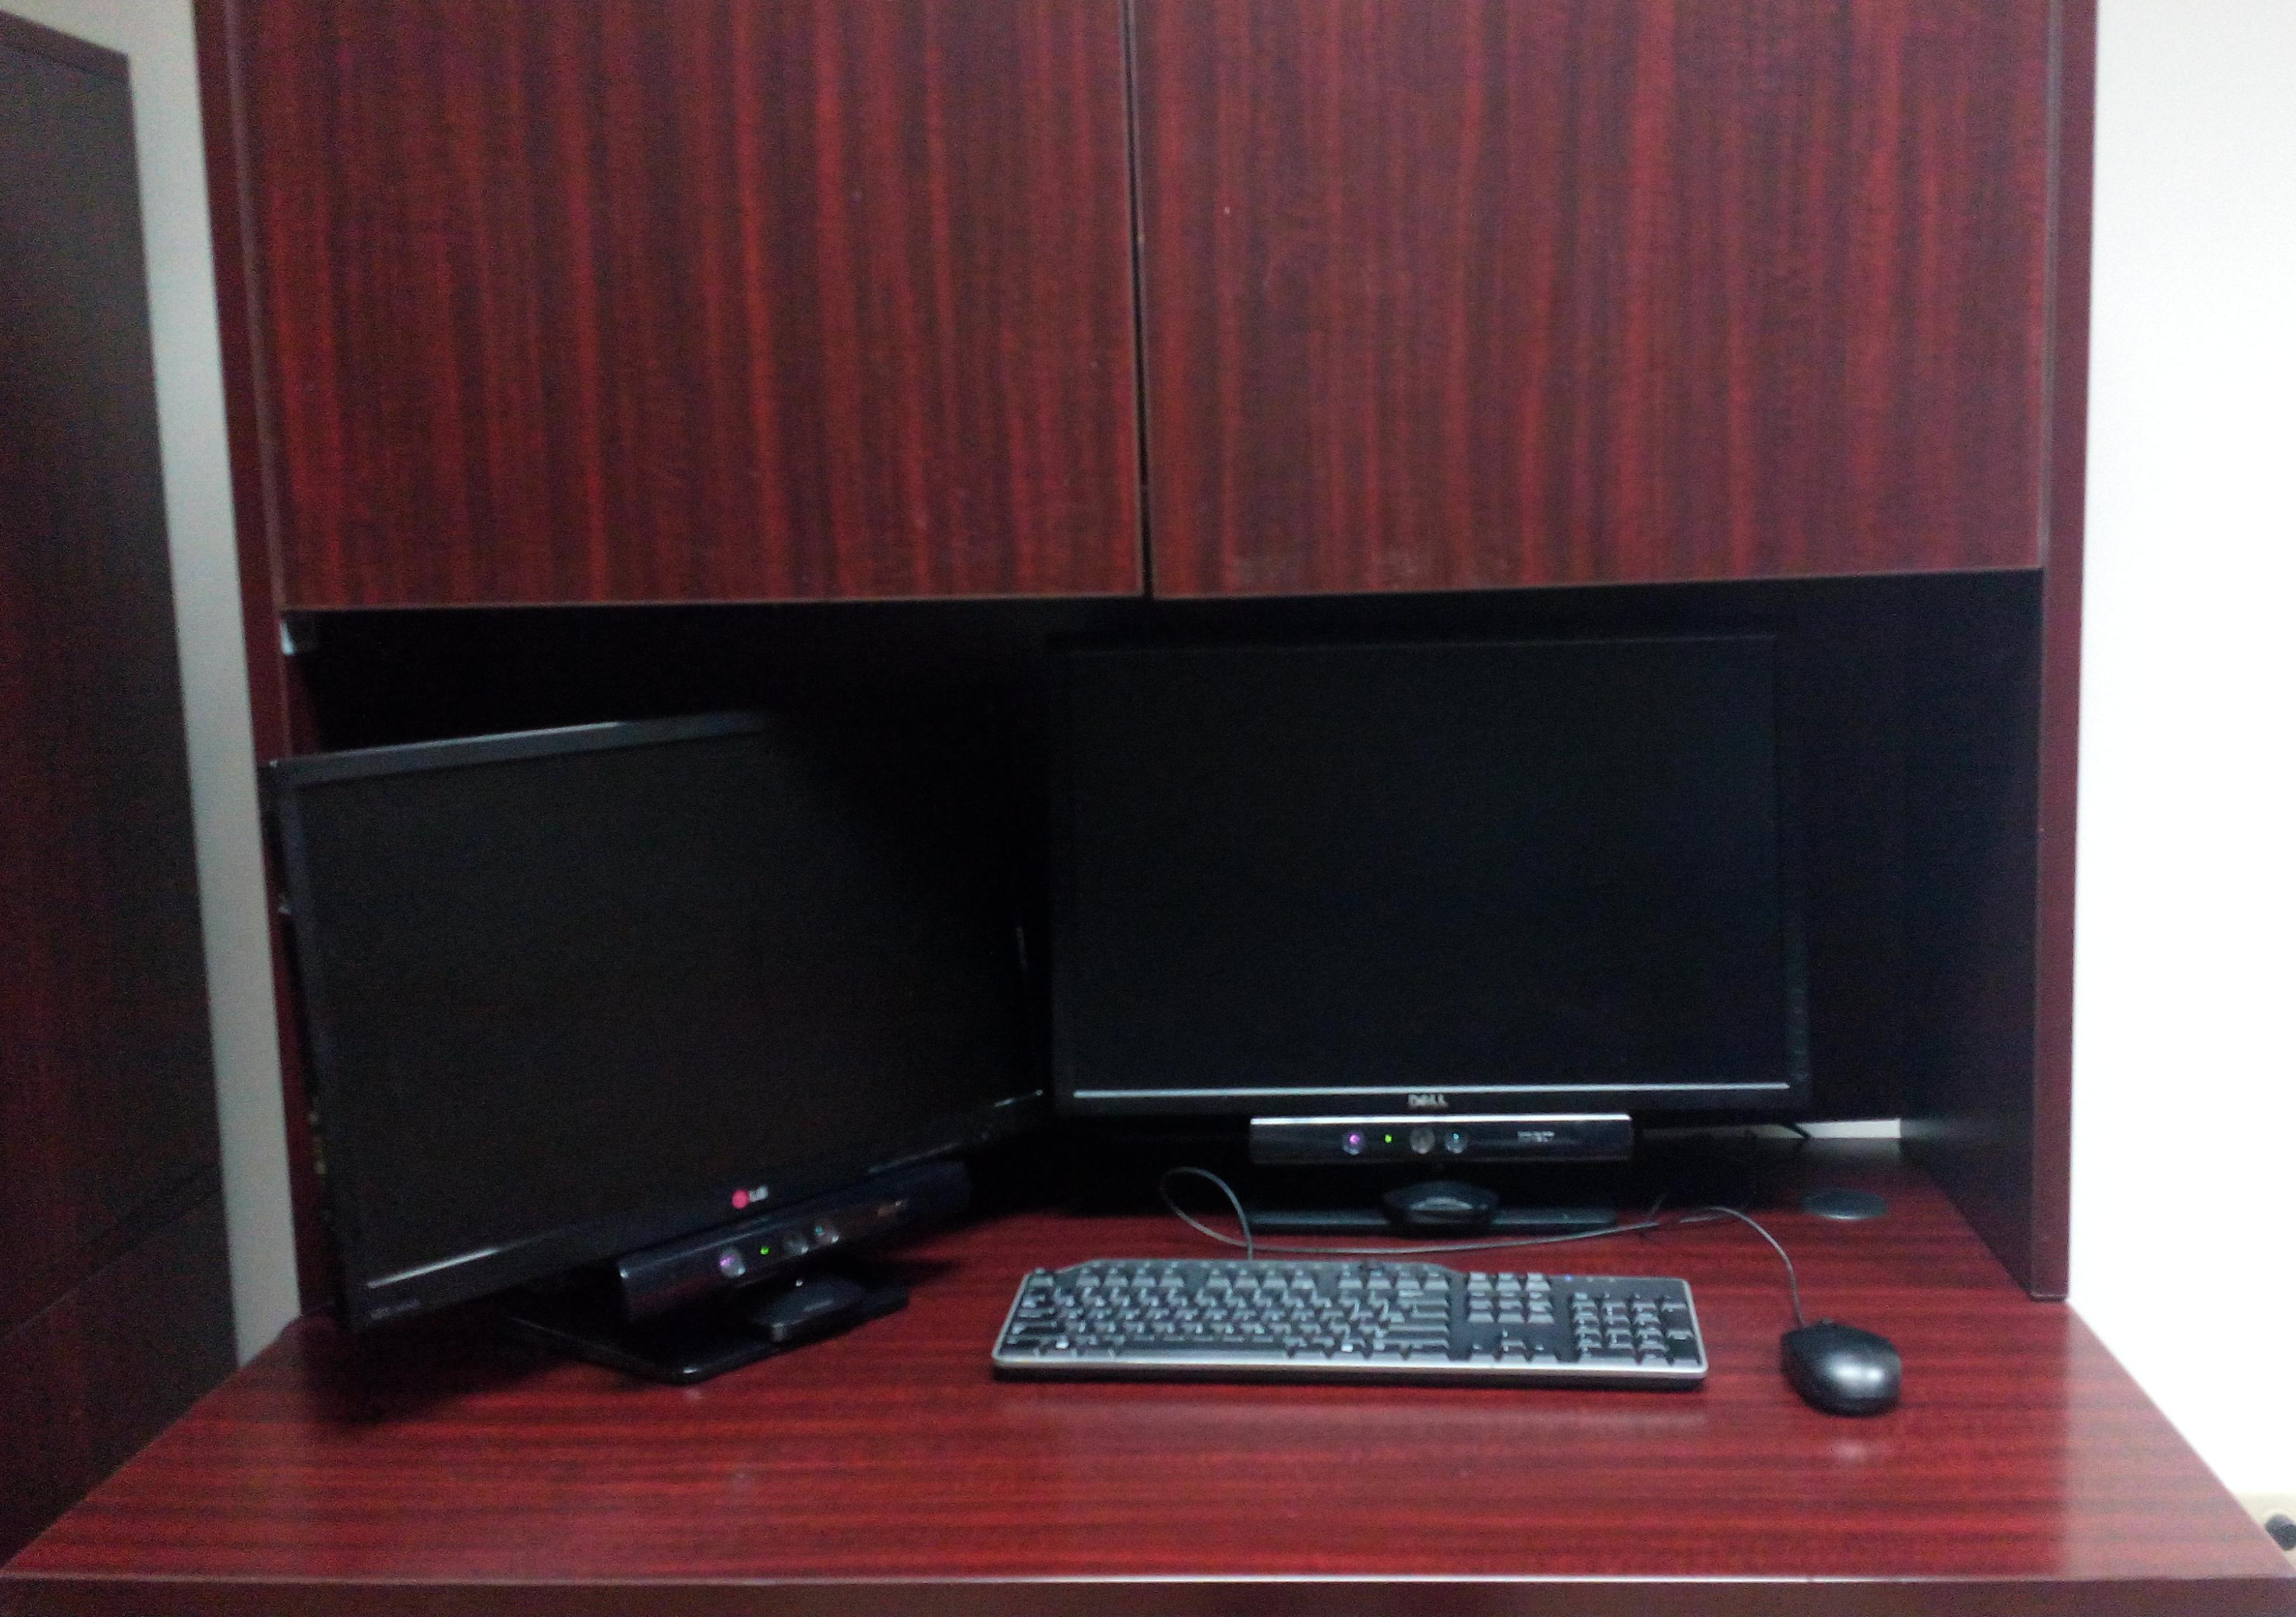
\includegraphics[scale=0.09]{./Figures/iluminacion.jpg}
\end{center}
\caption{Laboratorio en condiciones estándar de iluminación.}
\label{fig:LabIluminado}
\end{figure} 

En el primer experimento el usuario esta a una distancia de $70$ $cm.$ del Kinect frontal. Se muestra un ejemplo de las imágenes obtenidas de un usuario, para las imágenes de los demás usuarios ver el apéndice . En la tabla se encuentran los resultados del reconocimiento de los dos gestos.  

%\begin{figure}[h!]
%\centering
%\subfigure[Gesto 1 vista desde el Kinect frontal]{
\includegraphics[scale=.3]{./Figures/pusheen}\label{fig:iluminacion70:1}}
%\subfigure[Gesto 1 viata desde el Kinect lateral]{
\includegraphics[scale=.3]{./Figures/pusheen}\label{fig:iluminacion70:2}}
%\subfigure[Gesto 2 vista desde Kinect frontal]{
\includegraphics[scale=.3]{./Figures/pusheen}\label{fig:iluminacion70:3}}
%\subfigure[Gesto 2 vista desde Kinect lateral]{
\includegraphics[scale=.3]{./Figures/pusheen}\label{fig:iluminacion70:4}}
%\caption{Ejemplo de la imagenes capturadas a una distancia de $70$ $cm$.} \label{fig:iluminacion70}
%\end{figure}

\begin{table}[h!] 
\begin{center}
\begin{tabular}{ r || c | c |} 
 
        & Gesto 1 & Gesto 2 \\ \hline \hline  
Gesto 1 & 170  &  30  \\ \hline  
Gesto 2 & 21   & 179 \\   

\end{tabular}
\end{center} 
\caption{Matriz de confusión del experimento uno, utilizando ambos Kinect.}
\end{table}

\begin{table}[h!] 
\begin{center}
\begin{tabular}{ r || c | c |} 
 
        & Gesto 1 & Gesto 2 \\ \hline \hline  
Gesto 1 & 127  &  73  \\ \hline  
Gesto 2 & 6    &  194 \\   

\end{tabular}
\end{center} 
\caption{Matriz de confusión del experimento uno, utilizando solo el Kinect frontal.}
\end{table}
%----

En el segundo experimento el usuario esta a una distancia de $80$ $cm.$ del Kinect frontal. Se muestra un ejemplo de las imágenes obtenidas de un usuario. En la tabla se encuentran los resultados del reconocimiento de los dos gestos.   

%\begin{figure}[h!]
%\centering
%\subfigure[Gesto 1 vista desde el Kinect frontal]{
\includegraphics[scale=.3]{./Figures/pusheen}\label{fig:iluminacion80:1}}
%\subfigure[Gesto 1 viata desde el Kinect lateral]{
\includegraphics[scale=.3]{./Figures/pusheen}\label{fig:iluminacion80:2}}
%\subfigure[Gesto 2 vista desde Kinect frontal]{
\includegraphics[scale=.3]{./Figures/pusheen}\label{fig:iluminacion80:3}}
%\subfigure[Gesto 2 vista desde Kinect lateral]{
\includegraphics[scale=.3]{./Figures/pusheen}\label{fig:iluminacion80:4}}
%\caption{Ejemplo de la imagenes capturadas a una distancia de $80$ $cm$.} \label{fig:iluminacion80}
%\end{figure}

\begin{table}[h!] 
\begin{center}
\begin{tabular}{ r || c | c |} 
 
        & Gesto 1 & Gesto 2 \\ \hline \hline  
Gesto 1 & 96     &  104     \\ \hline  
Gesto 2 & 16     & 185     \\   

\end{tabular}
\end{center} 
\caption{Matriz de confusión del experimento dos, con dos Kinect} 
\end{table}

\begin{table}[h!] 
\begin{center}
\begin{tabular}{ r || c | c |} 
 
        & Gesto 1 & Gesto 2 \\ \hline \hline  
Gesto 1 & 88     &  112     \\ \hline  
Gesto 2 & 6     & 183     \\   

\end{tabular}
\end{center} 
\caption{Matriz de confusión del experimento dos, utilizando solo el Kinect frontal.} 
\end{table}

%---

En el tercer experimento el usuario esta a una distancia de $90$ $cm.$ del Kinect frontal. Se muestra un ejemplo de las imágenes obtenidas de un usuario. En la tabla se encuentran los resultados del reconocimiento de los dos gestos.    

%\begin{figure}[h!]
%\centering
%\subfigure[Gesto 1 vista desde el Kinect frontal]{
\includegraphics[scale=.3]{./Figures/pusheen}\label{fig:iluminacion90:1}}
%\subfigure[Gesto 1 viata desde el Kinect lateral]{
\includegraphics[scale=.3]{./Figures/pusheen}\label{fig:iluminacion90:2}}
%\subfigure[Gesto 2 vista desde Kinect frontal]{
\includegraphics[scale=.3]{./Figures/pusheen}\label{fig:iluminacion90:3}}
%\subfigure[Gesto 2 vista desde Kinect lateral]{
\includegraphics[scale=.3]{./Figures/pusheen}\label{fig:iluminacion90:4}}
%\caption{Ejemplo de la imagenes capturadas a una distancia de $90$ $cm$.} \label{fig:iluminacion70}
%\end{figure}

\begin{table}[h!] 
\begin{center}
\begin{tabular}{ r || c | c |} 
 
        & Gesto 1 & Gesto 2 \\ \hline \hline  
Gesto 1 &  93    & 107      \\ \hline  
Gesto 2 &  10    & 190     \\   

\end{tabular}
\end{center} 
\caption{Matriz de confusión, los datos se capturaron usando dos Kinect.}
\end{table}

\begin{table}[h!] 
\begin{center}
\begin{tabular}{ r || c | c |} 
 
        & Gesto 1 & Gesto 2 \\ \hline \hline  
Gesto 1 &  101   & 99      \\ \hline  
Gesto 2 &  17    & 183     \\   

\end{tabular}
\end{center} 
\caption{Matriz de confusión de los gestos 1 y 2. Utilizando un Kinect.}
\end{table} 

\subsection{Experimentos con iluminación media} 
Para el conjunto de estos experimentos, las imágenes se capturaron en un laboratorio con iluminación media, como la que se muestra en la figura. A tres distancias $70$, $80$ y $90$ $cm$.  

\begin{figure}[h!]
\begin{center} 
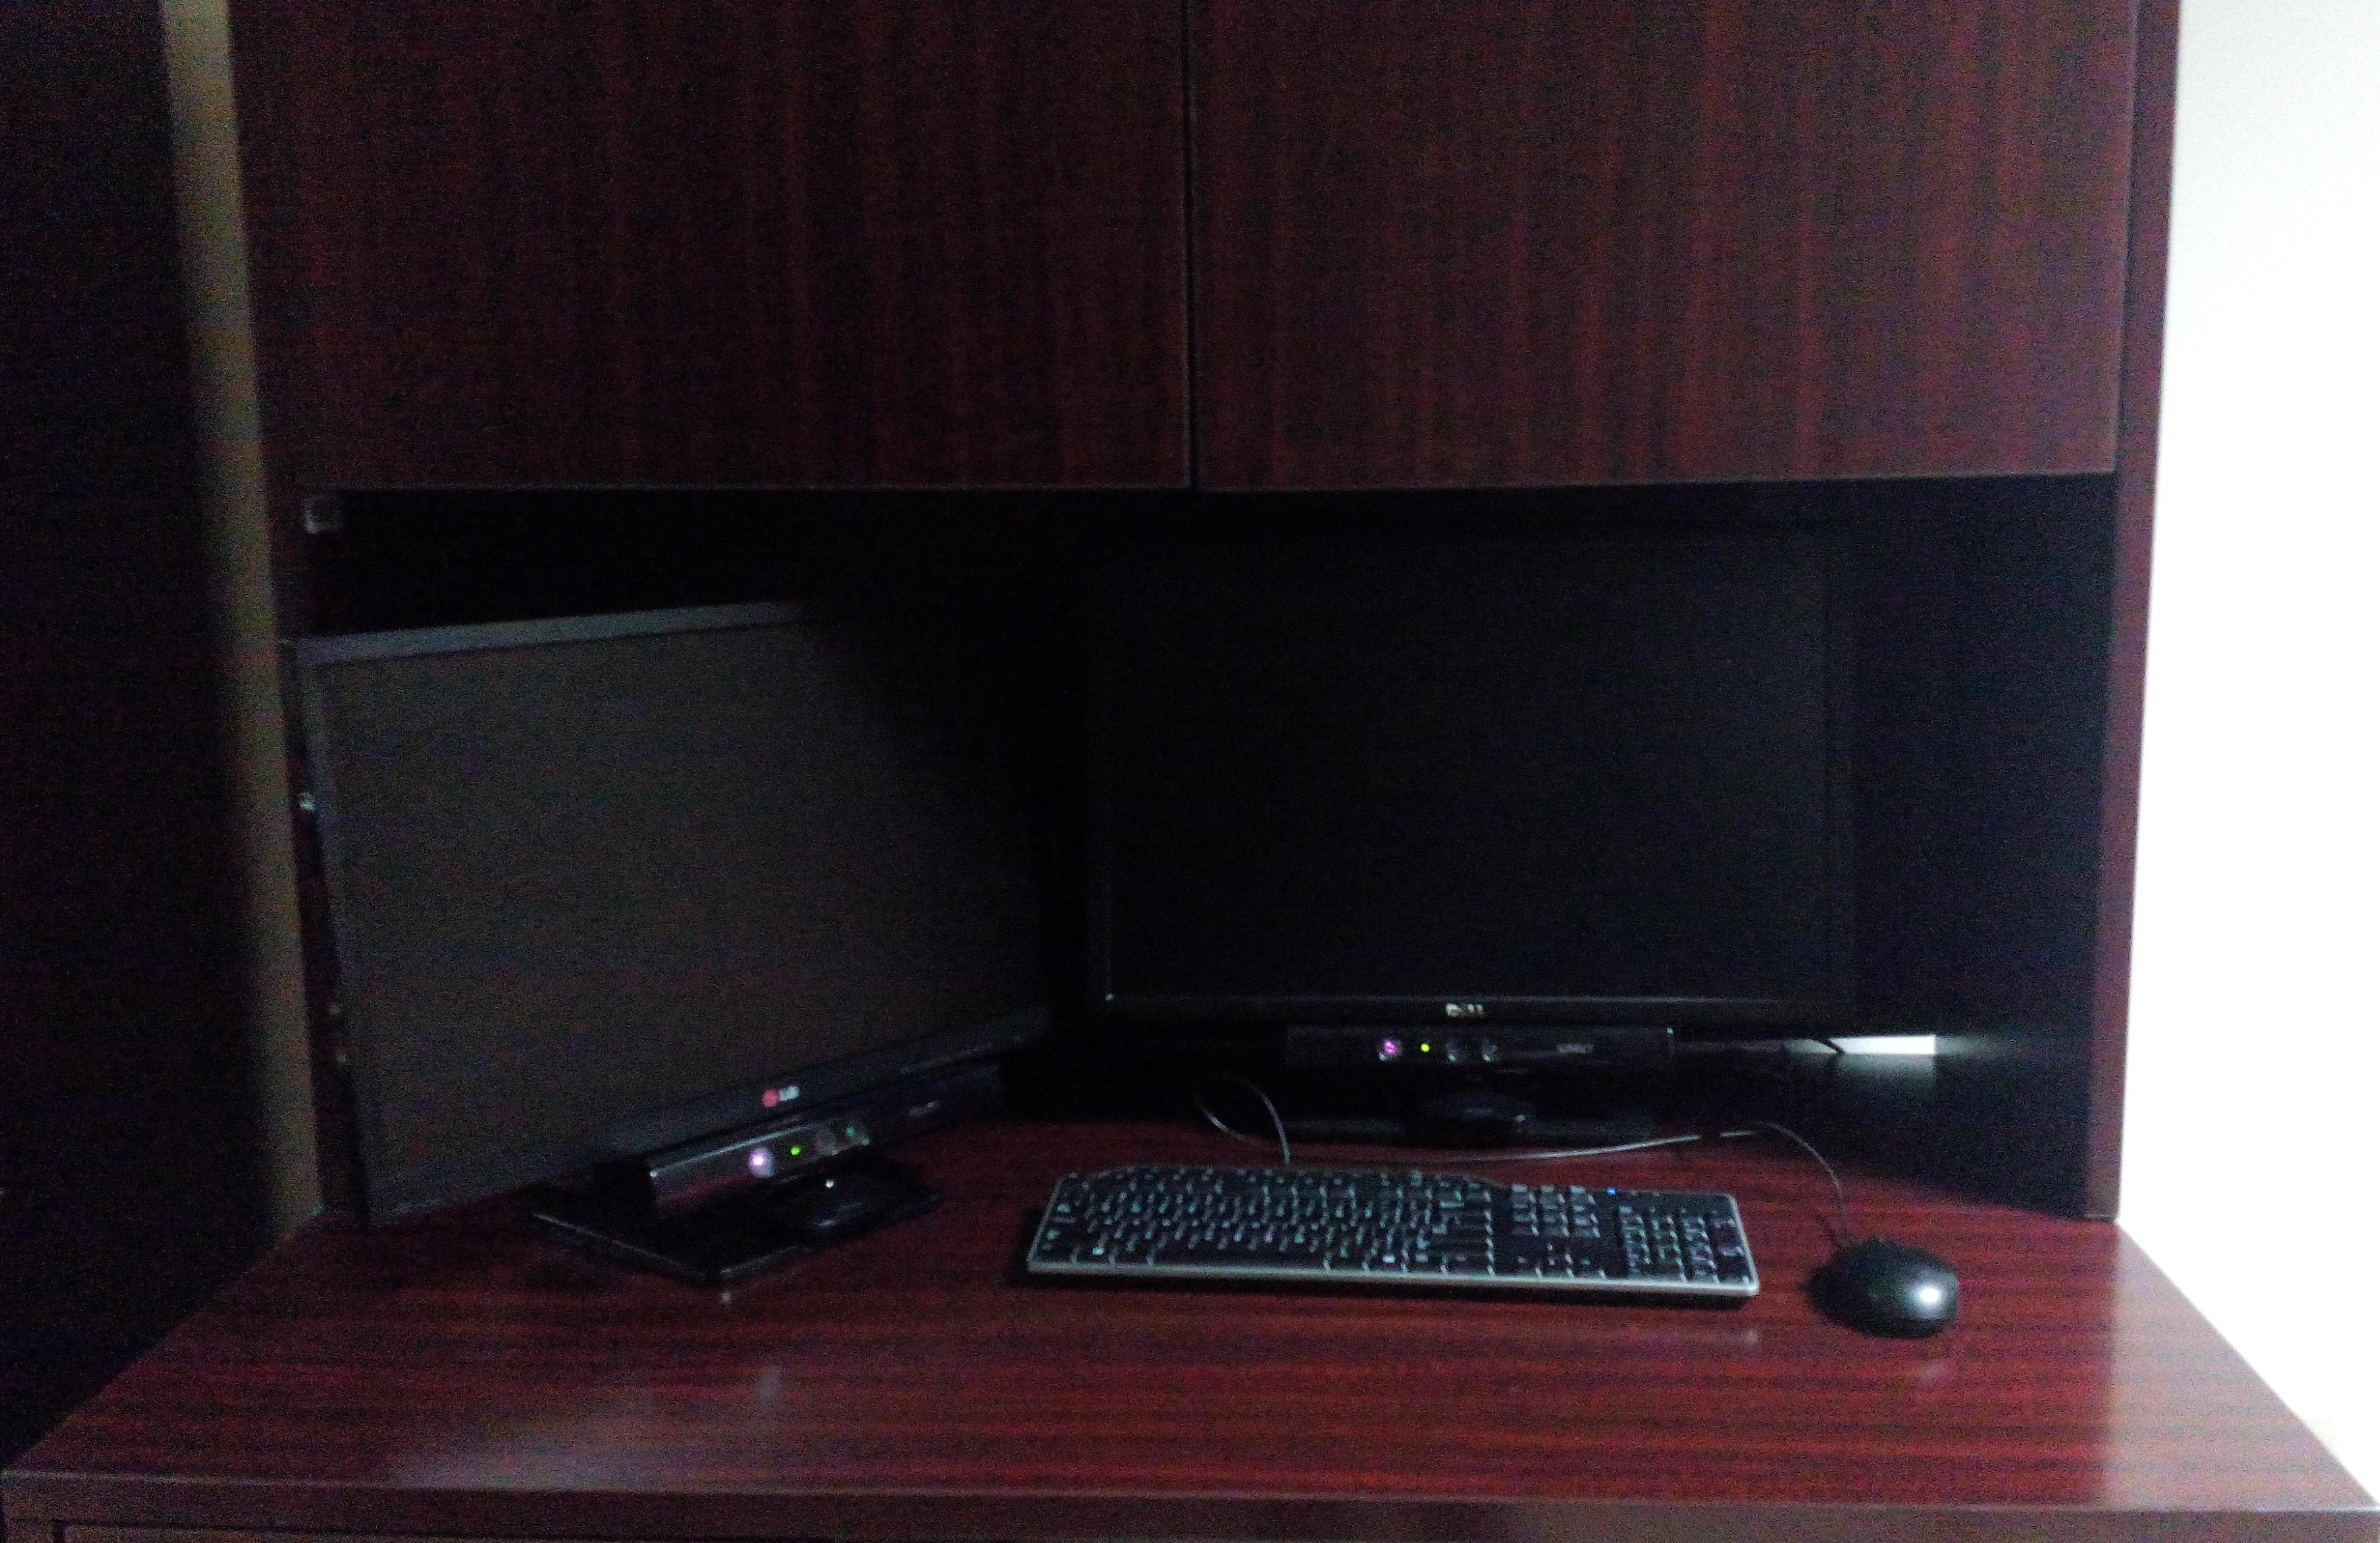
\includegraphics[scale=0.09]{./Figures/mediailuminacion.jpg}
\end{center}
\caption{Laboratorio en condiciones con iluminación media.}
\label{fig:LabMedioIluminado} 
\end{figure}  

%----

En el primer experimento el usuario esta a una distancia de $70$ $cm.$ del Kinect frontal. Se muestra un ejemplo de las imágenes obtenidas de un usuario. En la tabla se encuentran los resultados del reconocimiento de los dos gestos.  

%\begin{figure}[h!]
%\centering
%\subfigure[Gesto 1 vista desde el Kinect frontal]{
\includegraphics[scale=.3]{./Figures/pusheen}\label{fig:iluminacionM70:1}}
%\subfigure[Gesto 1 viata desde el Kinect lateral]{
\includegraphics[scale=.3]{./Figures/pusheen}\label{fig:iluminacionM70:2}}
%\subfigure[Gesto 2 vista desde Kinect frontal]{
\includegraphics[scale=.3]{./Figures/pusheen}\label{fig:iluminacionM70:3}}
%\subfigure[Gesto 2 vista desde Kinect lateral]{
\includegraphics[scale=.3]{./Figures/pusheen}\label{fig:iluminacionM70:4}}
%\caption{Ejemplo de la imagenes capturadas a una distancia de $70$ $cm$.} \label{fig:iluminacionM70}
%\end{figure}

\begin{table}[h!] 
\begin{center}
\begin{tabular}{ r || c | c |} 
 
        & Gesto 1 & Gesto 2 \\ \hline \hline  
Gesto 1 & 178    &  22     \\ \hline  
Gesto 2 & 84     & 105     \\   

\end{tabular}
\end{center} 
\caption{Matriz de confusión}
\end{table}


\begin{table}[h!] 
\begin{center}
\begin{tabular}{ r || c | c |} 
 
        & Gesto 1 & Gesto 2 \\ \hline \hline  
Gesto 1 & 136    &  64     \\ \hline  
Gesto 2 & 7     &  193     \\   

\end{tabular}
\end{center} 
\caption{Matriz de confusión. Se utilizo un Kinect para el análisis del reconocimiento}
\end{table}

%---

En el segundo experimento el usuario esta a una distancia de $80$ $cm.$ del Kinect frontal. Se muestra un ejemplo de las imágenes obtenidas de un usuario. En la tabla se encuentran los resultados del reconocimiento de los dos gestos.   

%\begin{figure}[h!]
%\centering
%\subfigure[Gesto 1 vista desde el Kinect frontal]{
\includegraphics[scale=.3]{./Figures/pusheen}\label{fig:iluminacionM80:1}}
%\subfigure[Gesto 1 viata desde el Kinect lateral]{
\includegraphics[scale=.3]{./Figures/pusheen}\label{fig:iluminacionM80:2}}
%\subfigure[Gesto 2 vista desde Kinect frontal]{
\includegraphics[scale=.3]{./Figures/pusheen}\label{fig:iluminacionM80:3}}
%\subfigure[Gesto 2 vista desde Kinect lateral]{
\includegraphics[scale=.3]{./Figures/pusheen}\label{fig:iluminacionM80:4}}
%\caption{Ejemplo de la imagenes capturadas a una distancia de $80$ $cm$.} \label{fig:iluminacionM80}
%\end{figure}

\begin{table}[h!] 
\begin{center}
\begin{tabular}{ r || c | c |} 
 
        & Gesto 1 & Gesto 2 \\ \hline \hline  
Gesto 1 &      &       \\ \hline  
Gesto 2 &      &     \\   

\end{tabular}
\end{center} 
\caption{Matriz de confusión}
\end{table} 

\begin{table}[h!] 
\begin{center}
\begin{tabular}{ r || c | c |} 
 
        & Gesto 1 & Gesto 2 \\ \hline \hline  
Gesto 1 &      &     \\ \hline  
Gesto 2 &      &     \\   

\end{tabular}
\end{center} 
\caption{Matriz de confusión, utilizando un Kinect} 
\end{table} 
 
%---

En el tercer experimento el usuario esta a una distancia de $90$ $cm.$ del Kinect frontal. Se muestra un ejemplo de las imágenes obtenidas de un usuario. En la tabla se encuentran los resultados del reconocimiento de los dos gestos.    

%\begin{figure}[h!]
%\centering
%\subfigure[Gesto 1 vista desde el Kinect frontal]{
\includegraphics[scale=.3]{./Figures/pusheen}\label{fig:iluminacionM90:1}}
%\subfigure[Gesto 1 viata desde el Kinect lateral]{
\includegraphics[scale=.3]{./Figures/pusheen}\label{fig:iluminacionM90:2}}
%\subfigure[Gesto 2 vista desde Kinect frontal]{
\includegraphics[scale=.3]{./Figures/pusheen}\label{fig:iluminacionM90:3}}
%\subfigure[Gesto 2 vista desde Kinect lateral]{
\includegraphics[scale=.3]{./Figures/pusheen}\label{fig:iluminacionM90:4}}
%\caption{Ejemplo de la imagenes capturadas a una distancia de $90$ $cm$.} \label{fig:iluminacionM90}
%\end{figure}

\begin{table}[h!] 
\begin{center}
\begin{tabular}{ r || c | c |} 
 
        & Gesto 1 & Gesto 2 \\ \hline \hline  
Gesto 1 & 153     &  47     \\ \hline  
Gesto 2 & 26      & 174     \\   

\end{tabular}
\end{center} 
\caption{Matriz de confusión}
\end{table}

\begin{table}[h!] 
\begin{center}
\begin{tabular}{ r || c | c |} 
 
        & Gesto 1 & Gesto 2 \\ \hline \hline  
Gesto 1 &  54    &   95    \\ \hline  
Gesto 2 &  0     &  0   \\   

\end{tabular}
\end{center} 
\caption{Matriz de confusión, utilizando un Kinect} 
\end{table}  

Para el análisis de uno y dos Kinect, como en todos los casos se analizaron las mismas imágenes. Debido a la posición de la mano solo se detectaron $149$ gestos de la clase uno y $0$ de la clase dos, cuando se utiliza el Kinect frontal.  


\subsection{Experimentos sin iluminación}
Para este experimento las imágenes se capturaron en un laboratorio sin iluminación, como la que se muestra en la figura.

\begin{figure}[h!]
\begin{center} 
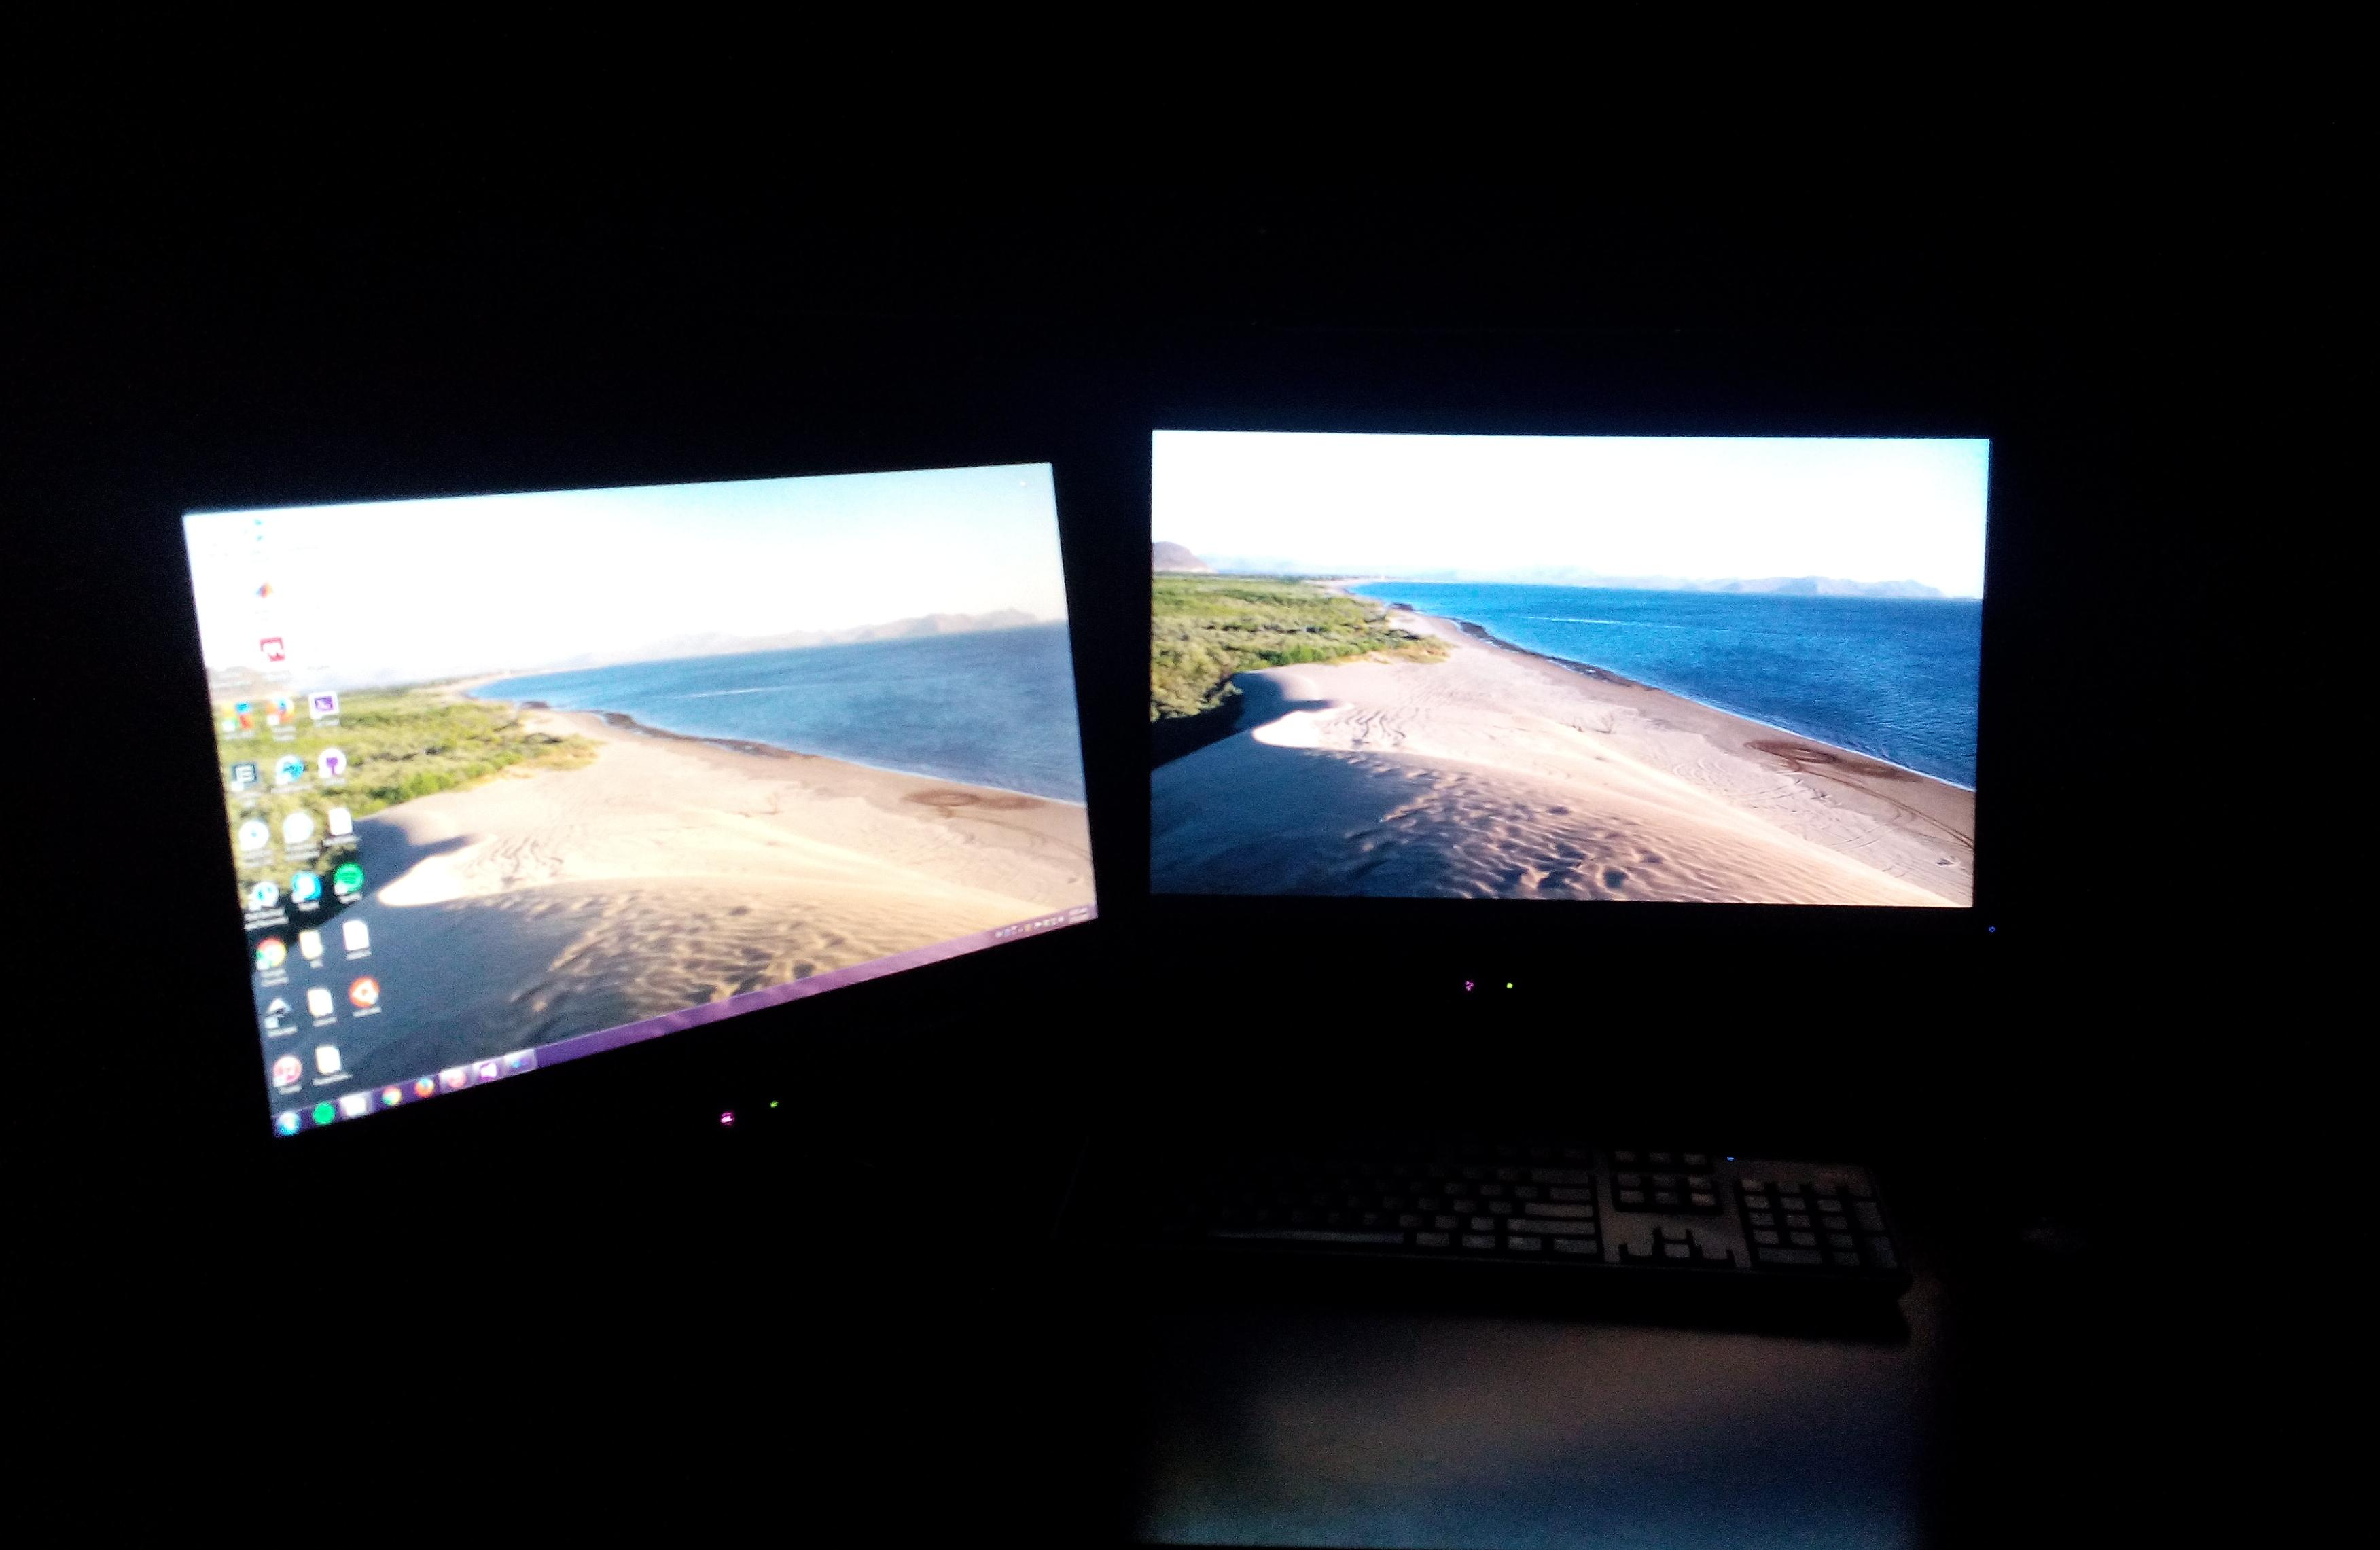
\includegraphics[scale=0.09]{./Figures/noIluminacion.jpg}
\end{center}
\caption{Laboratorio en condiciones con baja iluminación.}
\label{fig:LabNoIluminado} 
\end{figure} 

%---- 

En el primer experimento el usuario esta a una distancia de $70$ $cm.$ del Kinect frontal. Se muestra un ejemplo de las imágenes obtenidas de un usuario. En la tabla se encuentran los resultados del reconocimiento de los dos gestos.  

%\begin{figure}[h!]
%\centering
%\subfigure[Gesto 1 vista desde el Kinect frontal]{
\includegraphics[scale=.3]{./Figures/pusheen}\label{fig:iluminacionNo70:1}}
%\subfigure[Gesto 1 vista desde el Kinect lateral]{
\includegraphics[scale=.3]{./Figures/pusheen}\label{fig:iluminacionNo70:2}}
%\subfigure[Gesto 2 vista desde Kinect frontal]{
\includegraphics[scale=.3]{./Figures/pusheen}\label{fig:iluminacionNo70:3}}
%\subfigure[Gesto 2 vista desde Kinect lateral]{
\includegraphics[scale=.3]{./Figures/pusheen}\label{fig:iluminacionNo70:4}}
%\caption{Ejemplo de la imagenes capturadas a una distancia de $70$ $cm$.} \label{fig:iluminacionNo70}
%\end{figure}

\begin{table}[h!] 
\begin{center}
\begin{tabular}{ r || c | c |} 
 
        & Gesto 1 & Gesto 2 \\ \hline \hline  
Gesto 1 & 190     &  110     \\ \hline  
Gesto 2 & 196     &  4     \\   

\end{tabular}
\end{center} 
\caption{Matriz de confusión}
\end{table}  

\begin{table}[h!] 
\begin{center}
\begin{tabular}{ r || c | c |} 
 
        & Gesto 1 & Gesto 2 \\ \hline \hline  
Gesto 1 & 154     &  46     \\ \hline  
Gesto 2 & 167     &  33     \\   

\end{tabular}
\end{center} 
\caption{Matriz de confusión del reconocimiento de los dos gestos estáticos.}
\end{table} 


%----

En el segundo experimento el usuario esta a una distancia de $80$ $cm.$ del Kinect frontal. Se muestra un ejemplo de las imágenes obtenidas de un usuario. En la tabla se encuentran los resultados del reconocimiento de los dos gestos.   

%\begin{figure}[h!]
%\centering
%\subfigure[Gesto 1 vista desde el Kinect frontal]{
\includegraphics[scale=.3]{./Figures/pusheen}\label{fig:iluminacionNo80:1}}
%\subfigure[Gesto 1 vista desde el Kinect lateral]{
\includegraphics[scale=.3]{./Figures/pusheen}\label{fig:iluminacionNo80:2}}
%\subfigure[Gesto 2 vista desde Kinect frontal]{
\includegraphics[scale=.3]{./Figures/pusheen}\label{fig:iluminacionNo80:3}}
%\subfigure[Gesto 2 vista desde Kinect lateral]{
\includegraphics[scale=.3]{./Figures/pusheen}\label{fig:iluminacionNo80:4}}
%\caption{Ejemplo de la imagenes capturadas a una distancia de $80$ $cm$.} \label{fig:iluminacionNo80}
%\end{figure}

\begin{table}[h!] 
\begin{center}
\begin{tabular}{ r || c | c |} 
 
        & Gesto 1 & Gesto 2 \\ \hline \hline  
Gesto 1 & 187     &  13     \\ \hline  
Gesto 2 & 90     &  110     \\   

\end{tabular}
\end{center} 
\caption{Matriz de confusión}
\end{table}  

\begin{table}[h!] 
\begin{center}
\begin{tabular}{ r || c | c |} 
 
        & Gesto 1 & Gesto 2 \\ \hline \hline  
Gesto 1 & 162     &  37     \\ \hline  
Gesto 2 & 4     &  166     \\   

\end{tabular}
\end{center} 
\caption{Matriz de confusión del reconocimiento de los dos gestos estáticos.}
\end{table} 
\begin{center}
\begin{tabular}{ r || c | c |} 
 
        & Gesto 1 & Gesto 2 \\ \hline \hline  
Gesto 1 & 187     &  13     \\ \hline  
Gesto 2 & 90      & 110     \\   

\end{tabular}
\end{center} 
\caption{Matriz de confusión}
\end{table}

%---

En el tercer experimento el usuario esta a una distancia de $90$ $cm.$ del Kinect frontal. Se muestra un ejemplo de las imágenes obtenidas de un usuario. En la tabla se encuentran los resultados del reconocimiento de los dos gestos.    

%\begin{figure}[h!]
%\centering
%\subfigure[Gesto 1 vista desde el Kinect frontal]{
\includegraphics[scale=.3]{./Figures/pusheen}\label{fig:iluminacionNo90:1}}
%\subfigure[Gesto 1 viata desde el Kinect lateral]{
\includegraphics[scale=.3]{./Figures/pusheen}\label{fig:iluminacionNo90:2}}
%\subfigure[Gesto 2 vista desde Kinect frontal]{
\includegraphics[scale=.3]{./Figures/pusheen}\label{fig:iluminacionNo90:3}}
%\subfigure[Gesto 2 vista desde Kinect lateral]{
\includegraphics[scale=.3]{./Figures/pusheen}\label{fig:iluminacionNo90:4}}
%\caption{Ejemplo de la imagenes capturadas a una distancia de $90$ $cm$.} \label{fig:iluminacionNo70}
%\end{figure}

\begin{table}[h!] 
\begin{center}
\begin{tabular}{ r || c | c |} 
 
        & Gesto 1 & Gesto 2 \\ \hline \hline  
Gesto 1 & 150     &  50     \\ \hline  
Gesto 2 & 6      &  194     \\   

\end{tabular}
\end{center} 
\caption{Matriz de confusión}
\end{table}

\begin{table}[h!] 
\begin{center}
\begin{tabular}{ r || c | c |} 
 
        & Gesto 1 & Gesto 2 \\ \hline \hline  
Gesto 1 & 138     &  61     \\ \hline  
Gesto 2 & 0      &  0     \\   

\end{tabular}
\end{center} 
\caption{Matriz de confusión}
\end{table} 

No se detecto ningún elemento de la clase dos y solo se detectaron 98 elementos d ela primera clase. Debido que por la vista del kinect frontal no se pudo detectar la pose. 

Por las matrices anteriores se observa que hay un error mayor cuando se quieres identificar el gesto uno, esto debido a las imágenes provenientes del sensor, ya que no siempre es posible obtener una imagen completa de la mano, ni utilizando los dos dispositivos.  

%:::::::::::::::::::::::::::::::::::::::::::::::::::::::::::::::::::::::::::::::::::::::::::::::::::::::::::::::::


\section{Experimentos de gestos dinámicos}\label{TestDinamicGestures} 

La evaluación del sistema en cuanto al reconocimiento de los gestos dinámicos se realizo de la siguiente forma; al igual que en los gestos estáticos se hicieron dos conjuntos de experimentos cada uno con diferentes tipos de iluminación, media y sin iluminación. En cada conjunto de experimentos se tomo en cuenta la distancia, ya que en cada grupo se analizaron tres distancias, $70$, $80$, $90$ $cm$. 

Los gestos analizados fueron dos. El primero corresponde a la palma de la mano con los dedos separados, Gesto 3, en movimiento y el segundo el puño de la mano, Gesto 4, también en movimiento. Estos gestos fueron realizados por tres usuarios distintos. Para cada experimento se analizaron $150$ cuadros por lo que se analizaron $5$ repeticiones del gesto y cada uno tenia una duración de $30$ cuadros por segundo. Se tomo como gesto valido si el porcentaje de reconocimiento de cada gestos estático presente en cada segundo es mayor o igual a $80 \%$.  

Enseguida se presentan los resultados de cada experimento realizado, por usuario. También se presenta el rendimiento del sistema usando solo un solo Kinect. 

%\subsection{Experimentos con iluminación} 
%Para este experimento las imágenes se capturaron en un laboratorio con iluminación estándar,como la que se muestra en la figura \ref{fig:LabIluminado}.
%
%En el primer experimento el usuario esta a una distancia de $70$ $cm.$ del Kinect frontal. Se muestra un ejemplo de las imágenes obtenidas de un usuario, para las imágenes de los demás usuarios ver el apéndice . En la tabla se encuentran los resultados del reconocimiento de los dos gestos.  
%
%%\begin{figure}[h!]
%%\centering
%%\subfigure[Cuadro inicial]{
\includegraphics[scale=.3]{./Figures/pusheen}\label{fig:G1I70:1}}
%%\subfigure[Cuadro número 20]{
\includegraphics[scale=.3]{./Figures/pusheen}\label{fig:G1I70:2}}
%%\subfigure[Cuadro número 40]{
\includegraphics[scale=.3]{./Figures/pusheen}\label{fig:G1I70:3}}
%%\subfigure[Cuadro final]{
\includegraphics[scale=.3]{./Figures/pusheen}\label{fig:G1I70:4}}
%%\caption{Gesto de la palma con los dedos abiertas a $70$ $cm$.} \label{fig:G1I70}
%%\end{figure}
%%
%%\begin{figure}[h!]
%%\centering
%%\subfigure[Cuadro inicial]{
\includegraphics[scale=.3]{./Figures/pusheen}\label{fig:G2I70:1}}
%%\subfigure[Cuadro número 20]{
\includegraphics[scale=.3]{./Figures/pusheen}\label{fig:G2I70:2}}
%%\subfigure[Cuadro número 40]{
\includegraphics[scale=.3]{./Figures/pusheen}\label{fig:G2I70:3}}
%%\subfigure[Cuadro final]{
\includegraphics[scale=.3]{./Figures/pusheen}\label{fig:G2I70:4}}
%%\caption{Gesto del puño de la mano a $70$ $cm$.} \label{fig:G2I70}
%%\end{figure}
%
%
%
%%---
%
%En el segundo experimento el usuario esta a una distancia de $80$ $cm.$ del Kinect frontal. Se muestra un ejemplo de las imágenes obtenidas de un usuario. En la tabla se encuentran los resultados del reconocimiento de los dos gestos.   
%
%%\begin{figure}[h!]
%%\centering
%%\subfigure[Cuadro inicial]{
\includegraphics[scale=.3]{./Figures/pusheen}\label{fig:G1I80:1}}
%%\subfigure[Cuadro número 20]{
\includegraphics[scale=.3]{./Figures/pusheen}\label{fig:G1I80:2}}
%%\subfigure[Cuadro número 40]{
\includegraphics[scale=.3]{./Figures/pusheen}\label{fig:G1I80:3}}
%%\subfigure[Cuadro final]{\includegraphics[scale=.3]{./Figures/pusheen}\label{fig:G1I80:4}}
%%\caption{Gesto de la palma con los dedos abiertas a $80$ $cm$.} \label{fig:G1I80}
%%\end{figure}
%%
%%\begin{figure}[h!]
%%\centering
%%\subfigure[Cuadro inicial]{\includegraphics[scale=.3]{./Figures/pusheen}\label{fig:G2I80:1}}
%%\subfigure[Cuadro número 20]{\includegraphics[scale=.3]{./Figures/pusheen}\label{fig:G2I80:2}}
%%\subfigure[Cuadro número 40]{\includegraphics[scale=.3]{./Figures/pusheen}\label{fig:G2I80:3}}
%%\subfigure[Cuadro final]{\includegraphics[scale=.3]{./Figures/pusheen}\label{fig:G2I80:4}}
%%\caption{Gesto del puño de la mano a $80$ $cm$.} \label{fig:G2I0}
%%\end{figure}
%
%% 1 kinect 70 LM  
%\begin{tabular}{ |l|l|l|l|l|l|l| }
%\hline
%\multicolumn{7}{ |c| }{70 LM}\\ \cline{1-7}
%\multicolumn{2}{ |c| }{} &R1 & R2 & R3 & R4  & R5\\ \cline{1-7} \hline\hline
%{\multirow{2}{*}{P1}} & {G3} & 77 & 80 & 83 & 73 & 70 \\ \cline{2-7}
%                      & {G4} & 93 & 100 & 100 & 93 & 97 \\ \hline \hline
%{\multirow{2}{*}{P2}} & {G3} & 87 & 80 & 87 & 70 & 97 \\ \cline{2-7}
%                      & {G4} & 97 & 93 & 97 & 93 & 93 \\ \hline \hline
%{\multirow{2}{*}{P3}} & {G3} & 83 & 100 & 80 & 53 & 90 \\ \cline{2-7}
%                      & {G4} & 100 & 93 & 93 & 87 & 100 \\ \hline
%\end{tabular}\\\\
%
%%--- 
%
%En el tercer experimento el usuario esta a una distancia de $90$ $cm.$ del Kinect frontal. Se muestra un ejemplo de las imágenes obtenidas de un usuario. En la tabla se encuentran los resultados del reconocimiento de los dos gestos.    
%
%\begin{figure}[h!]
%\centering
%\subfigure[Cuadro inicial]{\includegraphics[scale=.3]{./Figures/pusheen}\label{fig:G1I90:1}}
%\subfigure[Cuadro número 20]{\includegraphics[scale=.3]{./Figures/pusheen}\label{fig:G1I90:2}}
%\subfigure[Cuadro número 40]{\includegraphics[scale=.3]{./Figures/pusheen}\label{fig:G1I90:3}}
%\subfigure[Cuadro final]{\includegraphics[scale=.3]{./Figures/pusheen}\label{fig:G1I90:4}}
%\caption{Gesto de la palma con los dedos abiertas $90$ $cm$.} \label{fig:G1I90}
%\end{figure}
%
%\begin{figure}[h!]
%\centering
%\subfigure[Cuadro inicial]{\includegraphics[scale=.3]{./Figures/pusheen}\label{fig:G2I90:1}}
%\subfigure[Cuadro número 20]{\includegraphics[scale=.3]{./Figures/pusheen}\label{fig:G2I90:2}}
%\subfigure[Cuadro número 40]{\includegraphics[scale=.3]{./Figures/pusheen}\label{fig:G2I90:3}}
%\subfigure[Cuadro final]{\includegraphics[scale=.3]{./Figures/pusheen}\label{fig:G2I90:4}}
%\caption{Gesto del puño de la mano $90$ $cm$.} \label{fig:G2I90}
%\end{figure}
%
%%\begin{tabular} { c c c }
%% cell1 & cell2 & cell3 \\ 
%% cell4 & cell5 & cell6 \\  
%% cell7 & cell8 & cell9    
%%\end{tabular}
%
%

\subsection{Experimentos con iluminación media} 
Para el conjunto de estos experimentos, las imágenes se capturaron en un laboratorio con iluminación media, como la que se muestra en la figura.

En el primer experimento el usuario esta a una distancia de $70$ $cm.$ del Kinect frontal. Se muestra un ejemplo de las imágenes obtenidas de un usuario, para las imágenes de los demás usuarios ver el apéndice. En la tabla se encuentran los resultados del reconocimiento de los dos gestos y por usuario.  

%\begin{figure}[h!]
%\centering
%\subfigure[Cuadro inicial]{\includegraphics[scale=.3]{./Figures/pusheen}\label{fig:G1IM70:1}}
%\subfigure[Cuadro número 20]{\includegraphics[scale=.3]{./Figures/pusheen}\label{fig:G1IM70:2}}
%\subfigure[Cuadro número 40]{\includegraphics[scale=.3]{./Figures/pusheen}\label{fig:G1IM70:3}}
%\subfigure[Cuadro final]{\includegraphics[scale=.3]{./Figures/pusheen}\label{fig:G1IM70:4}}
%\caption{Gesto de la palma con los dedos abiertas a $70$ $cm$.} \label{fig:G1IM70}
%\end{figure}
%
%\begin{figure}[h!]
%\centering
%\subfigure[Cuadro inicial]{\includegraphics[scale=.3]{./Figures/pusheen}\label{fig:G2IM70:1}}
%\subfigure[Cuadro número 20]{\includegraphics[scale=.3]{./Figures/pusheen}\label{fig:G2IM70:2}}
%\subfigure[Cuadro número 40]{\includegraphics[scale=.3]{./Figures/pusheen}\label{fig:G2IM70:3}}
%\subfigure[Cuadro final]{\includegraphics[scale=.3]{./Figures/pusheen}\label{fig:G2IM70:4}}
%\caption{Gesto del puño de la mano a $70$ $cm$.} \label{fig:G2IM70}
%\end{figure}

\begin{tabular}{ |l|l|l|l|l|l|l| }
\hline
\multicolumn{7}{ |c| }{Porcentajes de reconocimiento en cada secuencia de 30 seg. 1 Kinect}\\ \cline{1-7}
\multicolumn{2}{ |c| }{} &R1 & R2 & R3 & R4  & R5\\ \cline{1-7} \hline\hline
{\multirow{2}{*}{P1}} & {G3} & 77 & 80 & 83 & 73 & 70 \\ \cline{2-7}
                      & {G4} & 93 & 100 & 100 & 93 & 97 \\ \hline \hline
{\multirow{2}{*}{P2}} & {G3} & 87 & 80 & 87 & 70 & 97 \\ \cline{2-7}
                      & {G4} & 97 & 93 & 97 & 93 & 93 \\ \hline \hline
{\multirow{2}{*}{P3}} & {G3} & 83 & 100 & 80 & 53 & 90 \\ \cline{2-7}
                      & {G4} & 100 & 93 & 93 & 87 & 100 \\ \hline
\end{tabular}\\

\begin{tabular}{ |l|l|l|l|l|l|l| }
\hline
\multicolumn{7}{ |c| }{Porcentajes de reconocimiento en cada secuencia de 30 seg. 2 Kinect}\\ \cline{1-7}
\multicolumn{2}{ |c| }{} &R1 & R2 & R3 & R4  & R5\\ \cline{1-7} \hline\hline
{\multirow{2}{*}{P1}} & {G3} & 73 & 63 & 77 & 73 & 63 \\ \cline{2-7}
                      & {G4} & 100 & 100 & 100 & 100 & 100 \\ \hline \hline
{\multirow{2}{*}{P2}} & {G3} & 100 & 93 & 87 & 93 & 87 \\ \cline{2-7}
                      & {G4} & 93 & 77 & 77 & 67 & 60 \\ \hline \hline
{\multirow{2}{*}{P3}} & {G3} & 100 & 100 & 93 & 97 & 93 \\ \cline{2-7}
                      & {G4} & 73 & 90 & 83 & 63 & 83 \\ \hline
\end{tabular}\\  

%---

En el segundo experimento el usuario esta a una distancia de $80$ $cm.$ del Kinect frontal. Se muestra un ejemplo de las imágenes obtenidas de un usuario. En la tabla se encuentran los resultados del reconocimiento de los dos gestos.   

%\begin{figure}[h!]
%\centering
%\subfigure[Cuadro inicial]{\includegraphics[scale=.3]{./Figures/pusheen}\label{fig:G1IM80:1}}
%\subfigure[Cuadro número 20]{\includegraphics[scale=.3]{./Figures/pusheen}\label{fig:G1IM80:2}}
%\subfigure[Cuadro número 40]{\includegraphics[scale=.3]{./Figures/pusheen}\label{fig:G1IM80:3}}
%\subfigure[Cuadro final]{\includegraphics[scale=.3]{./Figures/pusheen}\label{fig:G1IM80:4}}
%\caption{Gesto de la palma con los dedos abiertas a $80$ $cm$.} \label{fig:G1I80}
%\end{figure}
%
%\begin{figure}[h!]
%\centering
%\subfigure[Cuadro inicial]{\includegraphics[scale=.3]{./Figures/pusheen}\label{fig:G2IM80:1}}
%\subfigure[Cuadro número 20]{\includegraphics[scale=.3]{./Figures/pusheen}\label{fig:G2IM80:2}}
%\subfigure[Cuadro número 40]{\includegraphics[scale=.3]{./Figures/pusheen}\label{fig:G2IM80:3}}
%\subfigure[Cuadro final]{\includegraphics[scale=.3]{./Figures/pusheen}\label{fig:G2IM80:4}}
%\caption{Gesto del puño de la mano a $80$ $cm$.} \label{fig:G2I80}
%\end{figure}

% 1 kinect 80 LM 
\begin{tabular}{ |l|l|l|l|l|l|l| }
\hline
\multicolumn{7}{ |c| }{Porcentajes de reconocimiento en cada secuencia de 30 seg. 1 Kinect}\\ \cline{1-7}
\multicolumn{2}{ |c| }{} &R1 & R2 & R3 & R4  & R5\\ \cline{1-7} \hline\hline
{\multirow{2}{*}{P1}} & {G3} & 33 & 27 & 30 & 50 & 57 \\ \cline{2-7}
                      & {G4} & 100 & 100 & 70 & 87 & 77 \\ \hline \hline
{\multirow{2}{*}{P2}} & {G3} & 37 & 27 & 33 & 38 & 29 \\ \cline{2-7}
                      & {G4} & 100 & 93 & 90 & 80 & 75 \\ \hline \hline
{\multirow{2}{*}{P3}} & {G3} & 47 & 87 & 60 & 60 & 63 \\ \cline{2-7}
                      & {G4} & 100 & 90 & 97 & 92 & 95 \\ \hline
\end{tabular}\\ 



\begin{tabular}{ |l|l|l|l|l|l|l| }
\hline
\multicolumn{7}{ |c| }{Porcentajes de reconocimiento en cada secuencia de 30 seg. 2 Kinect}\\ \cline{1-7}
\multicolumn{2}{ |c| }{} &R1 & R2 & R3 & R4  & R5\\ \cline{1-7} \hline\hline
{\multirow{2}{*}{P1}} & {G3} & 83 & 86 & 67 & 87 & 70 \\ \cline{2-7}
                      & {G4} & 35 & 53 & 70 & 77 & 57 \\ \hline \hline
{\multirow{2}{*}{P2}} & {G3} & 33 & 57 & 57 & 73 & 60 \\ \cline{2-7}
                      & {G4} & 93 & 93 & 90 & 90 & 80 \\ \hline \hline
{\multirow{2}{*}{P3}} & {G3} & 93 & 100 & 67 & 100 & 80 \\ \cline{2-7}
                      & {G4} & 100 & 93 & 87 & 83 & 90 \\ \hline
\end{tabular}\\


%---

En el tercer experimento el usuario esta a una distancia de $90$ $cm.$ del Kinect frontal. Se muestra un ejemplo de las imágenes obtenidas de un usuario. En la tabla se encuentran los resultados del reconocimiento de los dos gestos.    

%\begin{figure}[h!]
%\centering
%\subfigure[Cuadro inicial]{\includegraphics[scale=.3]{./Figures/pusheen}\label{fig:G1IM90:1}}
%\subfigure[Cuadro número 20]{\includegraphics[scale=.3]{./Figures/pusheen}\label{fig:G1IM90:2}}
%\subfigure[Cuadro número 40]{\includegraphics[scale=.3]{./Figures/pusheen}\label{fig:G1IM90:3}}
%\subfigure[Cuadro final]{\includegraphics[scale=.3]{./Figures/pusheen}\label{fig:G1IM90:4}}
%\caption{Gesto de la palma con los dedos abiertas $90$ $cm$.} \label{fig:G1IM90}
%\end{figure}
%
%\begin{figure}[h!]
%\centering
%\subfigure[Cuadro inicial]{\includegraphics[scale=.3]{./Figures/pusheen}\label{fig:G2IM90:1}}
%\subfigure[Cuadro número 20]{\includegraphics[scale=.3]{./Figures/pusheen}\label{fig:G2IM90:2}}
%\subfigure[Cuadro número 40]{\includegraphics[scale=.3]{./Figures/pusheen}\label{fig:G2IM90:3}}
%\subfigure[Cuadro final]{\includegraphics[scale=.3]{./Figures/pusheen}\label{fig:G2IM90:4}}
%\caption{Gesto del puño de la mano $90$ $cm$.} \label{fig:G2IM90}
%\end{figure}


\begin{tabular}{ |l|l|l|l|l|l|l| }
\hline
\multicolumn{7}{ |c| }{Porcentajes de reconocimiento en cada secuencia de 30 seg. 1 Kinect}\\ \cline{1-7}
\multicolumn{2}{ |c| }{} &R1 & R2 & R3 & R4  & R5\\ \cline{1-7} \hline\hline
{\multirow{2}{*}{P1}} & {G3} & 87 & 87 & 53 & 87 & 67 \\ \cline{2-7}
                      & {G4} & 100 & 100 & 100 & 90 & 92 \\ \hline \hline
{\multirow{2}{*}{P2}} & {G3} & 87 & 87 & 90 & 93 & 80 \\ \cline{2-7}
                      & {G4} & 83 & 73 & 97 & 80 & 75 \\ \hline \hline
{\multirow{2}{*}{P3}} & {G3} & 90 & 97 & 97 & 100 & 90 \\ \cline{2-7}
                      & {G4} & 77 & 90 & 80 & 75 & 80 \\ \hline
\end{tabular}

\begin{tabular}{ |l|l|l|l|l|l|l| }
\hline
\multicolumn{7}{ |c| }{Porcentajes de reconocimiento en cada secuencia de 30 seg. 2 Kinect}\\ \cline{1-7}
\multicolumn{2}{ |c| }{} &R1 & R2 & R3 & R4  & R5\\ \cline{1-7} \hline\hline
{\multirow{2}{*}{P1}} & {G3} & 30 & 37 & 13 & 13 & 30 \\ \cline{2-7}
                      & {G4} & 100 & 98 & 95 & 100 & 98 \\ \hline \hline
{\multirow{2}{*}{P2}} & {G3} & 50 & 60 & 67 & 70 & 75 \\ \cline{2-7}
                      & {G4} & 77 & 78 & 75 & 80 & 70 \\ \hline \hline
{\multirow{2}{*}{P3}} & {G3} & 77 & 73 & 80 & 97 & 90 \\ \cline{2-7}
                      & {G4} & 77 & 90 & 91 & 80 & 75 \\ \hline
\end{tabular}


\subsection{Experimentos sin iluminación}
Para este experimento las imágenes se capturaron en un laboratorio sin iluminación, como la que se muestra en la figura.

En el primer experimento el usuario esta a una distancia de $70$ $cm.$ del Kinect frontal. Se muestra un ejemplo de las imágenes obtenidas de un usuario, para las imágenes de los demás usuarios ver el apéndice . En la tabla se encuentran los resultados del reconocimiento de los dos gestos.  

%\begin{figure}[h!]
%\centering
%\subfigure[Cuadro inicial]{\includegraphics[scale=.3]{./Figures/pusheen}\label{fig:G1INO70:1}}
%\subfigure[Cuadro número 20]{\includegraphics[scale=.3]{./Figures/pusheen}\label{fig:G1INO70:2}}
%\subfigure[Cuadro número 40]{\includegraphics[scale=.3]{./Figures/pusheen}\label{fig:G1INO70:3}}
%\subfigure[Cuadro final]{\includegraphics[scale=.3]{./Figures/pusheen}\label{fig:G1INO70:4}}
%\caption{Gesto de la palma con los dedos abiertas a $70$ $cm$.} \label{fig:G1INO70}
%\end{figure}
%
%\begin{figure}[h!]
%\centering
%\subfigure[Cuadro inicial]{\includegraphics[scale=.3]{./Figures/pusheen}\label{fig:G2INO70:1}}
%\subfigure[Cuadro número 20]{\includegraphics[scale=.3]{./Figures/pusheen}\label{fig:G2INO70:2}}
%\subfigure[Cuadro número 40]{\includegraphics[scale=.3]{./Figures/pusheen}\label{fig:G2INO70:3}}
%\subfigure[Cuadro final]{\includegraphics[scale=.3]{./Figures/pusheen}\label{fig:G2INO70:4}}
%\caption{Gesto del puño de la mano a $70$ $cm$.} \label{fig:G2INO70}
%\end{figure}


\begin{tabular}{ |l|l|l|l|l|l|l| }
\hline
\multicolumn{7}{ |c| }{Porcentajes de reconocimiento en cada secuencia de 30 seg. 1 Kinect}\\ \cline{1-7}
\multicolumn{2}{ |c| }{} &R1 & R2 & R3 & R4  & R5\\ \cline{1-7} \hline\hline
{\multirow{2}{*}{P1}} & {G3} & 77 & 80 & 57 & 70 & 60 \\ \cline{2-7}
                      & {G4} & 100 & 97 & 93 & 100 & 97 \\ \hline \hline
{\multirow{2}{*}{P2}} & {G3} & 97 & 57 & 80 & 53 & 87 \\ \cline{2-7}
                      & {G4} & 100 & 97 & 83 & 87 & 87 \\ \hline \hline
{\multirow{2}{*}{P3}} & {G3} & 73 & 43 & 43 & 47 & 60 \\ \cline{2-7}
                      & {G4} & 100 & 93 & 97 & 93 & 93 \\ \hline
\end{tabular}


\begin{tabular}{ |l|l|l|l|l|l|l| }
\hline
\multicolumn{7}{ |c| }{Porcentajes de reconocimiento en cada secuencia de 30 seg. 2 Kinect}\\ \cline{1-7}
\multicolumn{2}{ |c| }{} &R1 & R2 & R3 & R4  & R5\\ \cline{1-7} \hline\hline
{\multirow{2}{*}{P1}} & {G3} & 93 & 83 & 100 & 77 & 87 \\ \cline{2-7}
                      & {G4} & 100 & 100 & 97 & 97 & 100 \\ \hline \hline
{\multirow{2}{*}{P2}} & {G3} & 97 & 97 & 87 & 93 & 97 \\ \cline{2-7}
                      & {G4} & 80 & 93 & 90 & 97 & 97 \\ \hline \hline
{\multirow{2}{*}{P3}} & {G3} & 83 & 87 & 97 & 97 & 100 \\ \cline{2-7}
                      & {G4} & 100 & 97 & 93 & 87 & 90 \\ \hline
\end{tabular}


%---

En el segundo experimento el usuario esta a una distancia de $80$ $cm.$ del Kinect frontal. Se muestra un ejemplo de las imágenes obtenidas de un usuario. En la tabla se encuentran los resultados del reconocimiento de los dos gestos.   

%\begin{figure}[h!]
%\centering
%\subfigure[Cuadro inicial]{\includegraphics[scale=.3]{./Figures/pusheen}\label{fig:G1INO80:1}}
%\subfigure[Cuadro número 20]{\includegraphics[scale=.3]{./Figures/pusheen}\label{fig:G1INO80:2}}
%\subfigure[Cuadro número 40]{\includegraphics[scale=.3]{./Figures/pusheen}\label{fig:G1INOM80:3}}
%\subfigure[Cuadro final]{\includegraphics[scale=.3]{./Figures/pusheen}\label{fig:G1INO80:4}}
%\caption{Gesto de la palma con los dedos abiertas a $80$ $cm$.} \label{fig:G1NO80}
%\end{figure}
%
%\begin{figure}[h!]
%\centering
%\subfigure[Cuadro inicial]{\includegraphics[scale=.3]{./Figures/pusheen}\label{fig:G2INO80:1}}
%\subfigure[Cuadro número 20]{\includegraphics[scale=.3]{./Figures/pusheen}\label{fig:G2INO80:2}}
%\subfigure[Cuadro número 40]{\includegraphics[scale=.3]{./Figures/pusheen}\label{fig:G2INO80:3}}
%\subfigure[Cuadro final]{\includegraphics[scale=.3]{./Figures/pusheen}\label{fig:G2INO80:4}}
%\caption{Gesto del puño de la mano a $80$ $cm$.} \label{fig:G2INO80}
%\end{figure}


\begin{tabular}{ |l|l|l|l|l|l|l| }
\hline
\multicolumn{7}{ |c| }{Porcentajes de reconocimiento en cada secuencia de 30 seg. 1 Kinect}\\ \cline{1-7}
\multicolumn{2}{ |c| }{} &R1 & R2 & R3 & R4  & R5\\ \cline{1-7} \hline\hline
{\multirow{2}{*}{P1}} & {G3} & 57 & 63 & 60 & 63 & 63 \\ \cline{2-7}
                      & {G4} & 100 & 100 & 100 & 100 & 100 \\ \hline \hline
{\multirow{2}{*}{P2}} & {G3} & 40 & 43 & 60 & 70 & 75 \\ \cline{2-7}
                      & {G4} & 100 & 93 & 97 & 93 & 98 \\ \hline \hline
{\multirow{2}{*}{P3}} & {G3} & 80 & 87 & 67 & 77 & 63 \\ \cline{2-7}
                      & {G4} & 97 & 87 & 100 & 90 & 87 \\ \hline
\end{tabular}\\

\begin{tabular}{ |l|l|l|l|l|l|l| }
\hline
\multicolumn{7}{ |c| }{Porcentajes de reconocimiento en cada secuencia de 30 seg. 2 Kinect}\\ \cline{1-7}
\multicolumn{2}{ |c| }{} &R1 & R2 & R3 & R4  & R5\\ \cline{1-7} \hline\hline
{\multirow{2}{*}{P1}} & {G3} & 63 & 70 & 90 & 80 & 77 \\ \cline{2-7}
                      & {G4} & 87 & 100 & 93 & 90 & 93 \\ \hline \hline
{\multirow{2}{*}{P2}} & {G3} & 60 & 73 & 47 & 63 & 73 \\ \cline{2-7}
                      & {G4} & 100 & 97 & 87 & 90 & 90 \\ \hline \hline
{\multirow{2}{*}{P3}} & {G3} & 87 & 100 & 73 & 83 & 80 \\ \cline{2-7}
                      & {G4} & 73 & 73 & 93 & 83 & 93 \\ \hline 
\end{tabular}

%--

En el tercer experimento el usuario esta a una distancia de $90$ $cm.$ del Kinect frontal. Se muestra un ejemplo de las imágenes obtenidas de un usuario. En la tabla se encuentran los resultados del reconocimiento de los dos gestos.    

%\begin{figure}[h!]
%\centering
%\subfigure[Cuadro inicial]{\includegraphics[scale=.3]{./Figures/pusheen}\label{fig:G1INO90:1}}
%\subfigure[Cuadro número 20]{\includegraphics[scale=.3]{./Figures/pusheen}\label{fig:G1INO90:2}}
%\subfigure[Cuadro número 40]{\includegraphics[scale=.3]{./Figures/pusheen}\label{fig:G1INO90:3}}
%\subfigure[Cuadro final]{\includegraphics[scale=.3]{./Figures/pusheen}\label{fig:G1INO90:4}}
%\caption{Gesto de la palma con los dedos abiertas $90$ $cm$.} \label{fig:G1INO90}
%\end{figure}
%
%\begin{figure}[h!]
%\centering
%\subfigure[Cuadro inicial]{\includegraphics[scale=.3]{./Figures/pusheen}\label{fig:G2INO90:1}}
%\subfigure[Cuadro número 20]{\includegraphics[scale=.3]{./Figures/pusheen}\label{fig:G2INO90:2}}
%\subfigure[Cuadro número 40]{\includegraphics[scale=.3]{./Figures/pusheen}\label{fig:G2INO90:3}}
%\subfigure[Cuadro final]{\includegraphics[scale=.3]{./Figures/pusheen}\label{fig:G2INO90:4}}
%\caption{Gesto del puño de la mano $90$ $cm$.} \label{fig:G2INO90}
%\end{figure}


\begin{tabular}{ |l|l|l|l|l|l|l| }
\hline
\multicolumn{7}{ |c| }{Porcentajes de reconocimiento en cada secuencia de 30 seg. 1 Kinect}\\ \cline{1-7}
\multicolumn{2}{ |c| }{} &R1 & R2 & R3 & R4  & R5\\ \cline{1-7} \hline\hline
{\multirow{2}{*}{P1}} & {G3} & 57 & 70 & 70 & 67 & 77 \\ \cline{2-7}
                      & {G4} &  &  &  &  &  \\ \hline \hline
{\multirow{2}{*}{P2}} & {G3} & 70 & 80 & 80 & 77 & 80 \\ \cline{2-7}
                      & {G4} & 73 & 80 & 83 & 97 & 80 \\ \hline \hline
{\multirow{2}{*}{P3}} & {G3} & 70 & 83 & 80 & 100 & 97 \\ \cline{2-7}
                      & {G4} & 87 & 97 & 90 & 70 & 90 \\ \hline
\end{tabular}



\begin{tabular}{ |l|l|l|l|l|l|l| }
\hline
\multicolumn{7}{ |c| }{Porcentajes de reconocimiento en cada secuencia de 30 seg. 2 Kinect}\\ \cline{1-7}
\multicolumn{2}{ |c| }{} &R1 & R2 & R3 & R4  & R5\\ \cline{1-7} \hline\hline
{\multirow{2}{*}{P1}} & {G3} & 47 & 47 & 53 & 37 & 40 \\ \cline{2-7}
                      & {G4} &  &  &  &  &  \\ \hline \hline
{\multirow{2}{*}{P2}} & {G3} & 37 & 63 & 63 & 75 & 80 \\ \cline{2-7}
                      & {G4} & 100 & 98 & 95 & 90 & 92 \\ \hline \hline
{\multirow{2}{*}{P3}} & {G3} & 80 & 97 & 87 & 83 & 87 \\ \cline{2-7}
                      & {G4} & 87 & 100 & 97 & 78 & 95 \\ \hline
\end{tabular}


En las tablas anteriores el gesto cuatro no pudo ser ubicado para el participante uno. 

Como se vio en cada tabla se analizo el porcentaje de gestos localizados en cada secuencia de $30$, analizando cuando se tenia uno y dos dispositivos. En general si se observa cada elemento o gesto, se puede observar que el sistema tienen un mayor grado de reconocimiento cuando se utilizan los dos dispositivos.    

También se observa que en algunas ocasiones el reconocimiento es bajo, usualmente para el gesto n\'umero tres, esto debido a la resolución de sensor, ya que en ocasiones las regiones de los dedos no son captadas y esto hace que reconozca erróneamente el gesto. 

La secuencia de imágenes de cada experimento fue procesa como provenía del sensor, no se escogieron las mejores imágenes. Los resultados prometen que con una mejor resolución del sensor el grado de reconocimiento seria mayor

%----------------------------------------------------------------------------------------------------------------------
%---------------------------------------------------------------------------------------------------------------------- 
\newpage